\chapter{Programación PLC}
\label{ch:progPLC}
Como se prensento en el capitulo \ref{ch:intro} de este informe el material a utilizar
para poder alcanzar los objetivos. En el presente capítulo se describe el algoritmo 
de programación del programa que se grabo en el \gls{plc}
\section{Algoritmo}
\label{sec:Algoritmo}



\usetikzlibrary{trees}
\tikzstyle{every node}=[draw=black,thick,anchor=west,inner sep=2pt,minimum size=1pt]
\tikzstyle{selected}=[draw=cyan,fill=cyan!30]
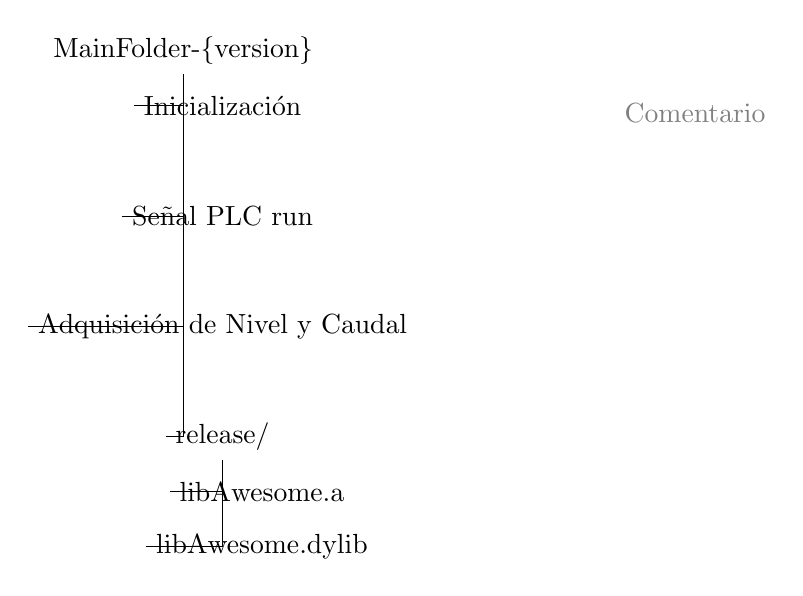
\begin{tikzpicture}[
  grow via three points={one child at (0.5,-0.7) and
  two children at (0.5,-0.7) and (0.5,-1.4)},   
  edge from parent path={(\tikzparentnode.south) |- (\tikzchildnode.west)}]
  \node {MainFolder-\{version\}}
    child { node [label={[xshift=6.0cm, yshift=-0.58cm, color=gray] Comentario}] {Inicialización}
        child [missing] {}
    }
    child [missing] {} %estos sirven para alinear.
    child { node {Señal PLC run}    }
    child [missing] {}
    child { node {Adquisición de Nivel y Caudal}    }
    child [missing] {}
    child { node {release/}
        child { node [draw=none] {libAwesome.a} }
        child { node [draw=none] {libAwesome.dylib} }
    };
\end{tikzpicture}
\tikzstyle{every node}=[] % resets borders of tables
\tikzstyle{selected}=[] % resets selected


\section{Programación}
\label{sec:Programacion}
Grabado y puesta en el plc

\begin{table}[!t]

\renewcommand{\arraystretch}{1.3}
\centering
\begin{tabular}{c||c}
\hline
\bfseries Memoria & \bfseries Descripción\\
\hline \hline
\verb|M0|  & Bandera de inicialización\\
\verb|M1|  & Lectura DP cell caudal\\
\verb|M2|  & Valor Kp\\
\verb|M3|  & Valor Ki\\
\verb|M4|  & Valor Kd\\
\hline
\end{tabular}
\caption{Banderas internas}
\end{table}

\begin{table}[!t]

\renewcommand{\arraystretch}{1.3}
\centering
\begin{tabular}{c||c||c||c}
\hline
\bfseries Tipo & \bfseries Word & \bfseries Bit & \bfseries Descripción\\
\hline \hline
Lect & \verb|MW0| & \verb|X0| & Señal Run PLC\\
Lect & & \verb|X1| & Alarma HHL\\
Lect & & \verb|X2|& Alarma LLL\\
Lect & & \verb|X3|& Alarma HL\\
Lect & & \verb|X4|& Alarma LL\\
Lect & & \verb|X5|& Error en motores (era \verb|MW0:X13|)\\
Lect & & \verb|X6|& Motor 1 encendido (era \verb|MW0:X11|)\\
Lect & & \verb|X7|& Motor 2 encendido(era \verb|MW0:X12|)\\
Lect & & \verb|X8|& Modo manual activado (era \verb|MW0:X14|)\\
Lect & & \verb|X9|& Modo automático activado y funcionando (Nuevo)\\
Lect & & \verb|X10|& Planta funcionando sin errores (era \verb|MW0:X15|)\\
\hline
Esc & \verb|MW1| & \verb|X0|& Switch modo manual/automático (era 
\verb|MW0:X10|)\\
Esc & & \verb|X1|& Aplicar (era \verb|MW0:X15|)\\
Esc & & \verb|X2|& Encender/Apagar (automático) (era \verb|MW0:X9|)\\
Esc & & \verb|X3|& Se desea cambiar el PID (era \verb|MW0:X6|)\\
Esc & & \verb|X4|& Se desean los valores por default para el PID (era 
\verb|MW0:X7|)\\
Esc & & \verb|X5|& Se desean valores por default para SP (era \verb|MW0:X8|)\\
Esc & & \verb|X6|& Encender M1 (manual) (era \verb|MW8:X1|)\\
Esc & & \verb|X7|& Encender M2 (manual) (era \verb|MW8:X2|)\\
Esc & & \verb|X8|& Limpiar errores (era \verb|MW8:X0|)\\
\hline

\hline
\end{tabular}
\caption{Bits lectura/escritura}
\end{table}

\begin{table}[!t]

\renewcommand{\arraystretch}{1.3}
\centering
\begin{tabular}{c||c||c}
\hline
\bfseries Tipo & \bfseries Word  & \bfseries Descripción\\
\hline \hline
Lect & \verb|MW2|  & Lectura DP cell nive (era \verb|MW1|)\\
Lect & \verb|MW3|  & Lectura DP cell caudal\\
Lect & \verb|MW4|  & Valor Kp\\
Lect & \verb|MW5|  & Valor Ki\\
Lect & \verb|MW6|  & Valor Kd\\
Lect & \verb|MW7|  & Valor de lectura del SP (era \verb|MW2|)\\
Lect & \verb|MW8|  & Valor de lectura de la válvula (era \verb|MW7|)\\
\hline
Esc & \verb|MW9| & Valor de escritura de la válvula (manual) (era 
\verb|MW15|) \\
Esc & \verb|MW10|  & Valor de escritura del SP \\
Esc & \verb|MW11|  & Valor de escritura Kp \\
Esc & \verb|MW12|  & Valor de escritura ki) \\
Esc & \verb|MW13| & Valor de escritura Kd \\
\hline
\end{tabular}
\caption{Palabras lectura/escritura}
\end{table}

\section{Depuración (Debug)}
\label{sec:Debug}
Forzar entradas
